% -*- root: ../main.tex -*-
\subsection{Implementierung}
Das Modell wurde zunächst mit Hilfe des Mapleskriptes ``GenerateFunktionJacobi.mw'' generiert. Dazu wurde zunächst die Funktion $f(x, u)$ sowie die Matrizen $A$ und $B$ wurden \ref{subsub:Jacobi} berechnet.  Die Matrizen $A$ und $D$ wurden durch die Umgruppierung $Bv:=[A_{1, 1}, \dotso, A_{13, 1}, A_{1, 2}, \dotso, A_{13, 2}, \dotso, A_{13, 13}]$ und $Bv:=[B_{1, 1}, \dotso B_{13, 1}, B_{1, 2}, \dotso, B_{13, 4}]$ in die Vektorform gebracht. Für das gesamte zu lösende Differentialgleichungssystem gilt nun: $[\dot{x}, \dot{Av}, \dot{Bv}]:=[f(x, u), Av, Bv] =: F \in \mathbb{R}^{234}$. Nach dem Lösen der ODE, können die Ergebnisse wieder zu Matrizen $\Phi_1, \Phi_2$ transformiert werden, um die Jacobimatrix $J:=[\Phi_1, \Phi_2]$ zu erhalten.\\
\\ 
Durch Analyse verschiedener Löser für gewöhnliche Differentialgleichungen in Matlab (ode45, ode23, ode15s, ode23s), wurde festgestellt, dass das System steif ist. Somit wird für die Lösung der ODE, die Jacobimatrix $J_F$ für $F$ benötigt, dazu wurde in MAPLE $F$ nach $x, Av, Bv$ abgeleitet. \\
\\
Abschließend wurde mit Hilfe des CodeGeneration Package von MAPLE C Code generiert und mit Hilfe der Pythonskripte ``GenerateScript.py'' und ``GenerateDyn.py'' Ersetzungen (Bsp.: Warnungen, Datentypen) durchgeführt und mit der Templatedatei ``rtopt\_gen.template'' in festgelegte Form gebracht. Die Ausgabe der Codegenerierung wird in die C - Datei ``rtopt\_gen.c'' geschrieben. Die generierten Funktionen werden durch die Wrapperfunktionen ``f'', ``jac'' in ``dyn.c'' aufgerufen. \\
\\
Zum Lösen der ODE wurden verschiedene Softwarepakete ausgetestet (Matlab, odeint, CVODE) mit verschiedenen Lösern (Matlab: ode45, ode15s, ode23s; odeint: rosenbrock4 ohne und mit cuda; CVODE: CV\_BDF, CV\_ADAMS). Als schnellster Löser/Methode hat sich die Methode CV\_ADAMS des Softwarepaketes CVODE von Alan. C. Hindmarsh herausgestellt \cite{Hindmarsh2015}. Die Methode ``integrate'' in ``solver.c'' ruft die Funktionen des Softwarepaketes auf und gibt als Ergebnis die Zustände $h(t_{x_k}, x_{k-1}, u_{k-1})$ sowie deren Jacobimatrix $J=[\Phi_1, \Phi_2]$ zurück.
\subsubsection{Parameterfindung}
Als nächster Schritt wurden realistische Parameter mit Hilfe des Softwaretools; GUI\_Modeling des Softwarepaket \href{https://github.com/dch33/Quad-Sim}{Quad-Sim} Quadrocopter gefunden:\\
\begin{tabular}[t]{|l|l|}
  \hline
  $m_{ges}$ & $\SI{1.022}{kg}$  \\ 
  $g$     & $\SI{9.81}{kg.s^{-2}}$  \\
  $I_{ges}$ & $\mathrm{diag}(0.0093886, 0.0093886, 0.018406)\, \mathrm{kg} \cdot \mathrm{m}^2$\\
  $kT$ & $\SI{1.5e-7}{N.{RPM}^{-2}}$\\
  $kQ$ & $\SI{3.0e-9}{N.m.{RPM}^{-2}}$\\
  $d$ & $\SI{0.22}{m}$\\
  $I_M$ & $\SI{4.4466e-6}{kg.m^2}$\\
  \hline
\end{tabular}\\
\begin{figure}[ht]
  \centering
  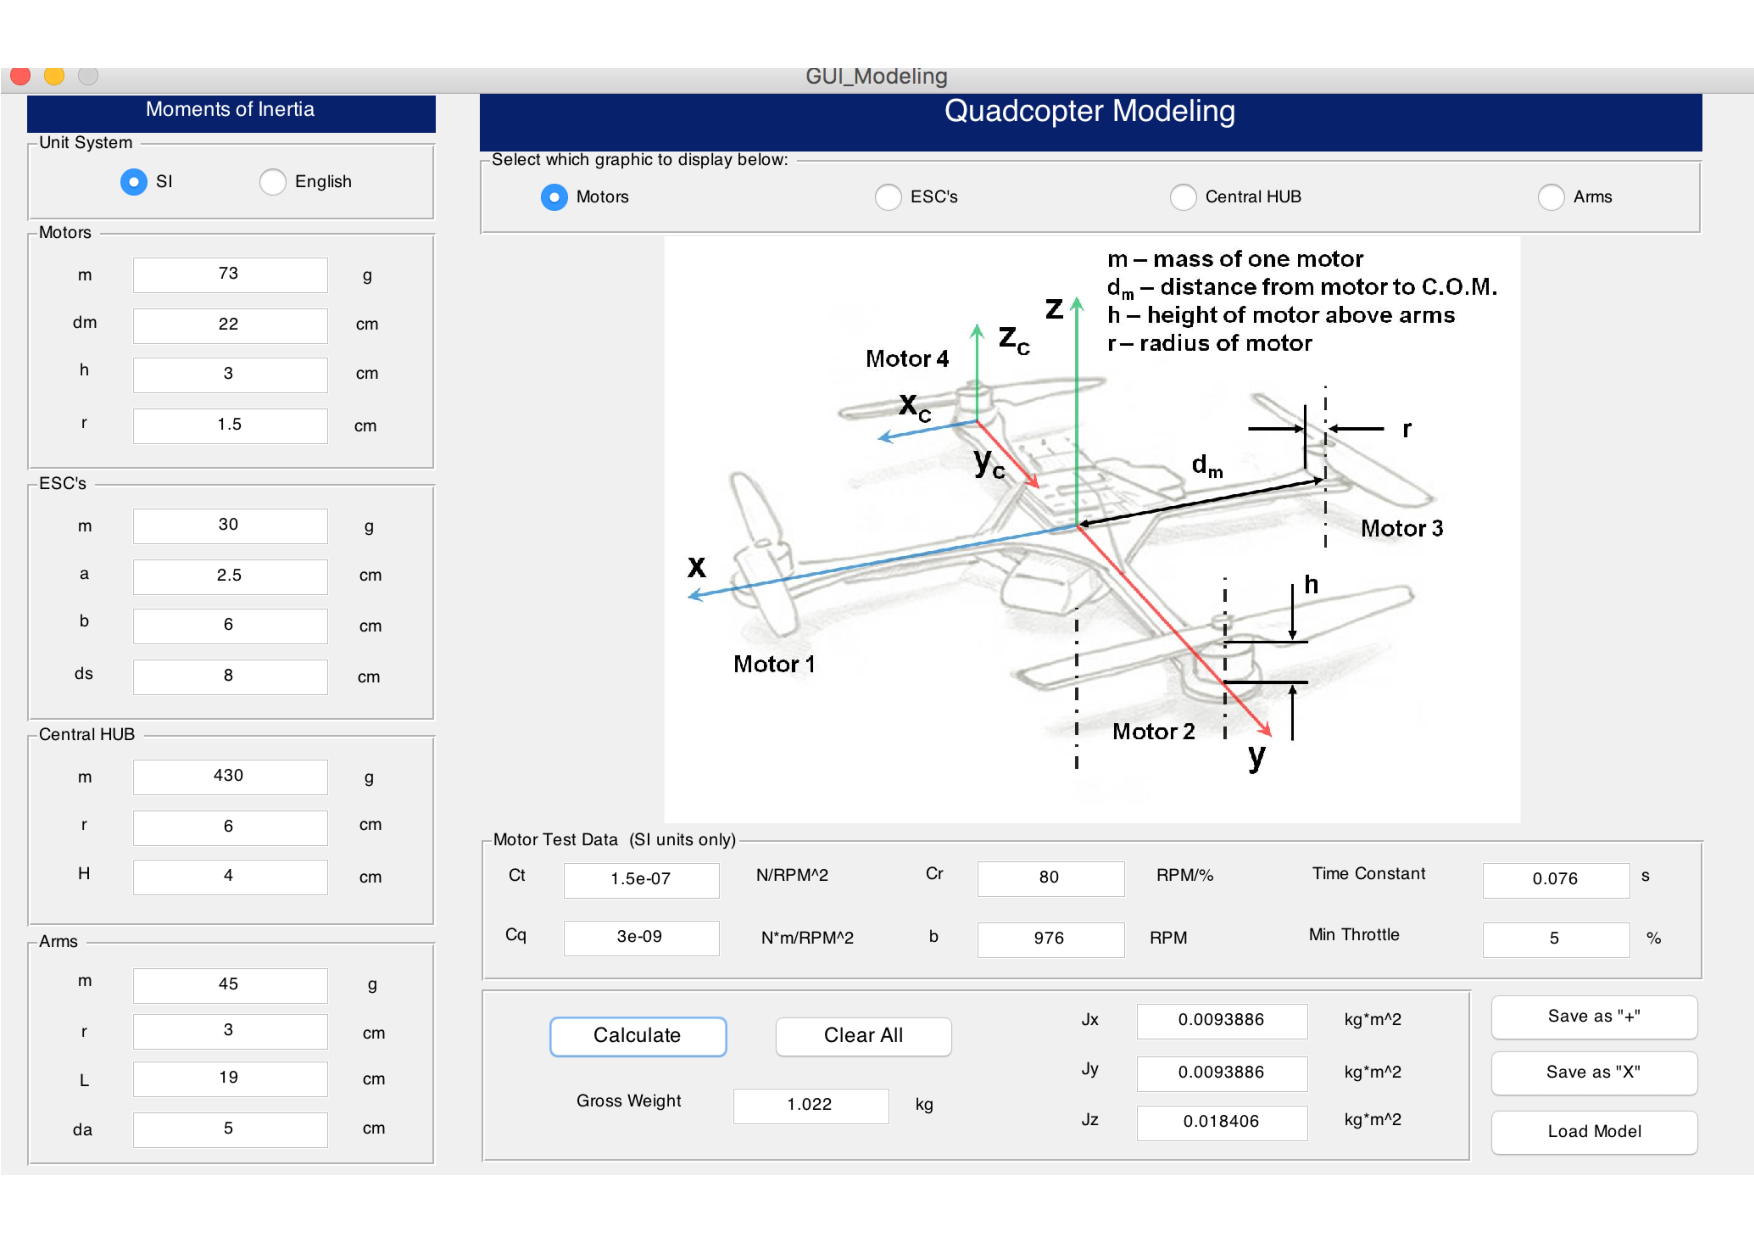
\includegraphics[width=\linewidth]{images/KonfigurationsManager.pdf}
  \caption{Konfigurationsmanager}
  \label{fig:konfigurationsmanager}
\end{figure} 
\subsubsection{Tests}
Um die Implementierung der Funktionen ``integrate'' und ``jac''zu ratifizieren wurden und die Testfunktionen ``numDiff\_nDvec'' in ``solver.c'' und ``testJac'' in ``dyn.c'' geschrieben. Für die Funktion ``integrate'' konnte nur ein qualitativer Test geschrieben werden, da die numerische Differenzierung zu ungenau für die exakte Lösung des nichtlinearen ODE System war.
